%% -*- Lecture -*-

\documentclass[11pt,aspectratio=169]{beamer}

\usepackage{rcstalk}
\usetheme{rcstheme}

\usepackage{tikz}
\usetikzlibrary{shapes,arrows,shadows,positioning,patterns,matrix,calc}
\usepackage{pgf}

\subtitle{Lecture 6: System Calls and Interrupts}
\topic{Processes, Threads and System Calls}

\begin{document}

\maketitle

\section{Kernel API}

\begin{slide}{System Software Stack}
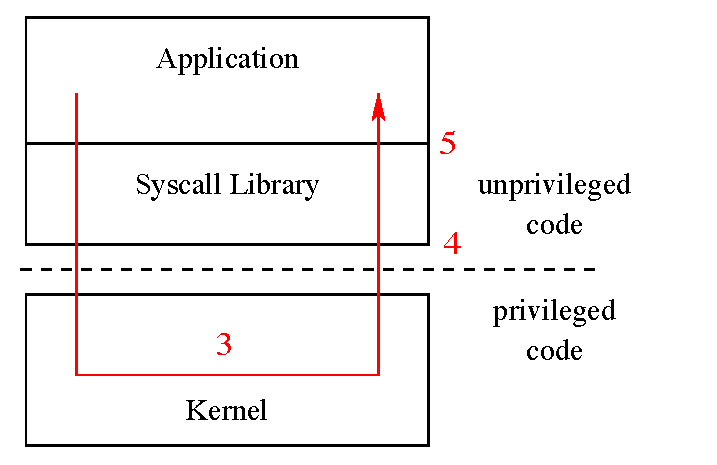
\includegraphics{osbound3.pdf}
\end{slide}

\begin{slide}{System Call Interface}
\begin{block}{}
{\em System Calls}: Application programmer interface (API) that 
    programmers use to interact with the operating system.
\end{block}
\itms{
\item Processes invoke system calls
\item Examples: \manp{fork}, \manp{waitpid}, \manp{open}, \manp{close}, 
    ...
\item System call interface can have complex calls
\ittms{
	\item \manp{sysctl} Exposes operating system configuration
	\item \manp{ioctl} Controlling devices
}
\item Need a mechanism to safely enter and exit the kernel
\ittms{
	\item Applications don't call kernel functions directly!
	\item Remember: kernels provide protection
}
}
\end{slide}

\begin{slide}{Privilege Modes}
\itms{
\item Hardware provides multiple protection modes% (or domains)
\item At least two modes:
\ittms{
\item {\em Kernel Mode} or {\em Privileged Mode} -- Operating System
\item {\em User Mode} -- Applications
}
\item Kernel Mode can access privileged CPU features
\ittms{
\item Access all restricted CPU features% (e.g., Coprocessor 0 on MIPS)
\item Enable/disable interrupts, setup interrupt handlers
\item Control system call interface
\item Modify the TLB (virtual memory ... future lecture)
}
\item Allows kernel to protect itself and isolate processes
\ittms{
\item Processes cannot read/write kernel memory
\item Processes cannot directly call kernel functions
}
}
\end{slide}

\begin{slide}{Mode Transitions}
\vspace{-1em}
\begin{columns}
\column{0.7\textwidth}
\itms{
\item Kernel Mode can only be entered through well defined entry points
\item Two classes of entry points provided by the processor:
\item {\em Interrupts}
\ittms{
\item Interrupts are generated by devices to signal needing attention
\item E.g. Keyboard input is ready
\item More on this during our IO lecture!
}
\item {\em Exceptions}:
\ittms{
\item Exceptions are caused by processor
\item E.g. Divide by zero, page faults, internal CPU errors
}
\item Interrupts and exceptions cause hardware to transfer control to the {\em 
	interrupt/exception handler}, a fixed entry point in the kernel.
}
\column{0.3\textwidth}
\end{columns}
\end{slide}

\begin{slide}{Interrupts}
\itms{
\item Interrupt are raised by devices
\item {\em Interrupt handler} is a function in the kernel that services a device 
	request
\item Interrupt Process:
\ittms{
\item Device signals the processor through a physical pin or bus message
\item Processor interrupts the current program
\item Processor begins executing the interrupt handler in privileged mode
}
\item Most interrupts can be disabled, but not all
\ittms{
\item Non-maskable interrupts (NMI) is for urgent system requests
}
}
\end{slide}

\begin{slide}{Exceptions}
\itms{
\item Exceptions (or faults) are conditions encountered during execution of a 
	program
\ittms{
\item Exceptions are due to multiple reasons:
\item Program Errors: Divide-by-zero, Illegal instructions
\item Operating System Requests: Page faults
\item Hardware Errors: System check (bad memory or internal CPU failures)
}
\item CPU handles exceptions similar to interrupts
\ittms{
\item Processor stops at the instruction that triggered the exception (usually)
\item Control is transferred to a fixed location where the exception handler is 
	located in privileged mode
}
\item System calls are a class of exceptions!
}
\end{slide}

\begin{slide}{x86-64 Exception Vectors}
\itms{
\item Interrupts, exceptions and system calls use the same mechanism
\item x86--64 offers a high performance path for system calls (not used in COS)
}
\begin{smallccode}
#define T_DE            0       /* Divide Error Exception */
#define T_DB            1       /* Debug Exception */
#define T_NMI           2       /* NMI Interrupt */
#define T_BP            3       /* Breakpoint Exception */
#define T_OF            4       /* Overflow Exception */
#define T_BR            5       /* BOUND Range Exceeded Exception */
#define T_UD            6       /* Invalid Opcode Exception */
#define T_NM            7       /* Device Not Available Exception */
#define T_DF            8       /* Double Fault Exception */
#define T_TS            10      /* Invalid TSS Exception */
#define T_NP            11      /* Segment Not Present */
#define T_SS            12      /* Stack Fault Exception */
#define T_GP            13      /* General Protection Exception */
#define T_PF            14      /* Page-Fault Exception */
#define T_MF            16      /* x87 FPU Floating-Point Error */
#define T_AC            17      /* Alignment Check Exception */
#define T_MC            18      /* Machine-Check Exception */
...
\end{smallccode}
\end{slide}

\begin{slide}{System Calls}
\itms{
\item System calls are performed by triggering the \texttt{T\_SYS} exception:
\gap
}
\begin{enumerate}
\item Application loads the arguments into CPU registers
\item Load the system call number into register \code{rdi} (first arg)
\item Executes \code{int 60} instruction to trigger \texttt{T\_SYS} exception
\item Processor looks up the interrupt vector
\item Processor jumps to the kernel exception handler
\item Returns to userspace using \code{iret}, return from exception instruction
\end{enumerate}
\end{slide}

\begin{slide}{Hardware Interrupt Handling in x86--64}
\itms{
\item Interrupt descriptor table: defines the entry point for interrupt 
    vector.
\item Configuring the IDT:
}
\begin{enumerate}
\item OS initializes IDT with entry point of interrupt vectors (1-255)
\end{enumerate}
\centerline{
    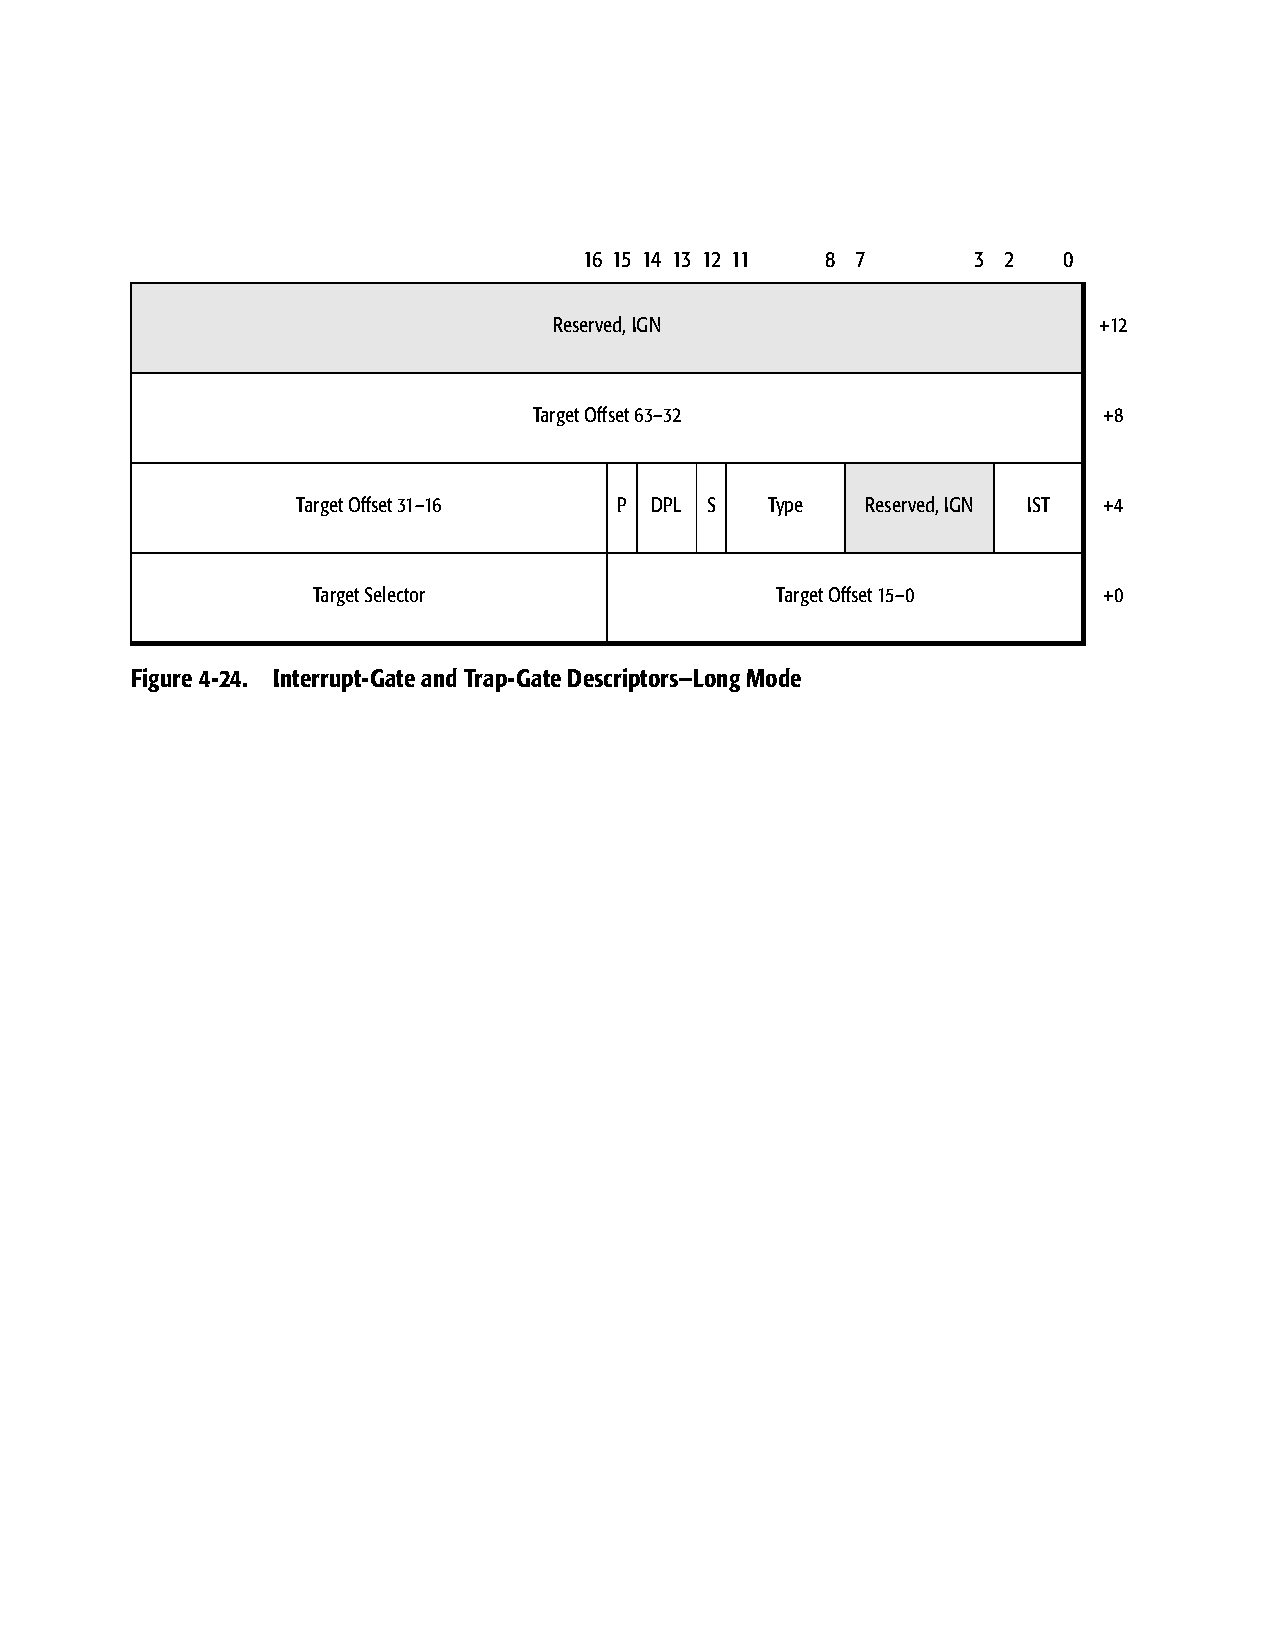
\includegraphics[height=50mm]{intgate.pdf}
}
\end{slide}

\begin{slide}{Interrupt Gate Descriptor (x86--64)}
\centerline{
    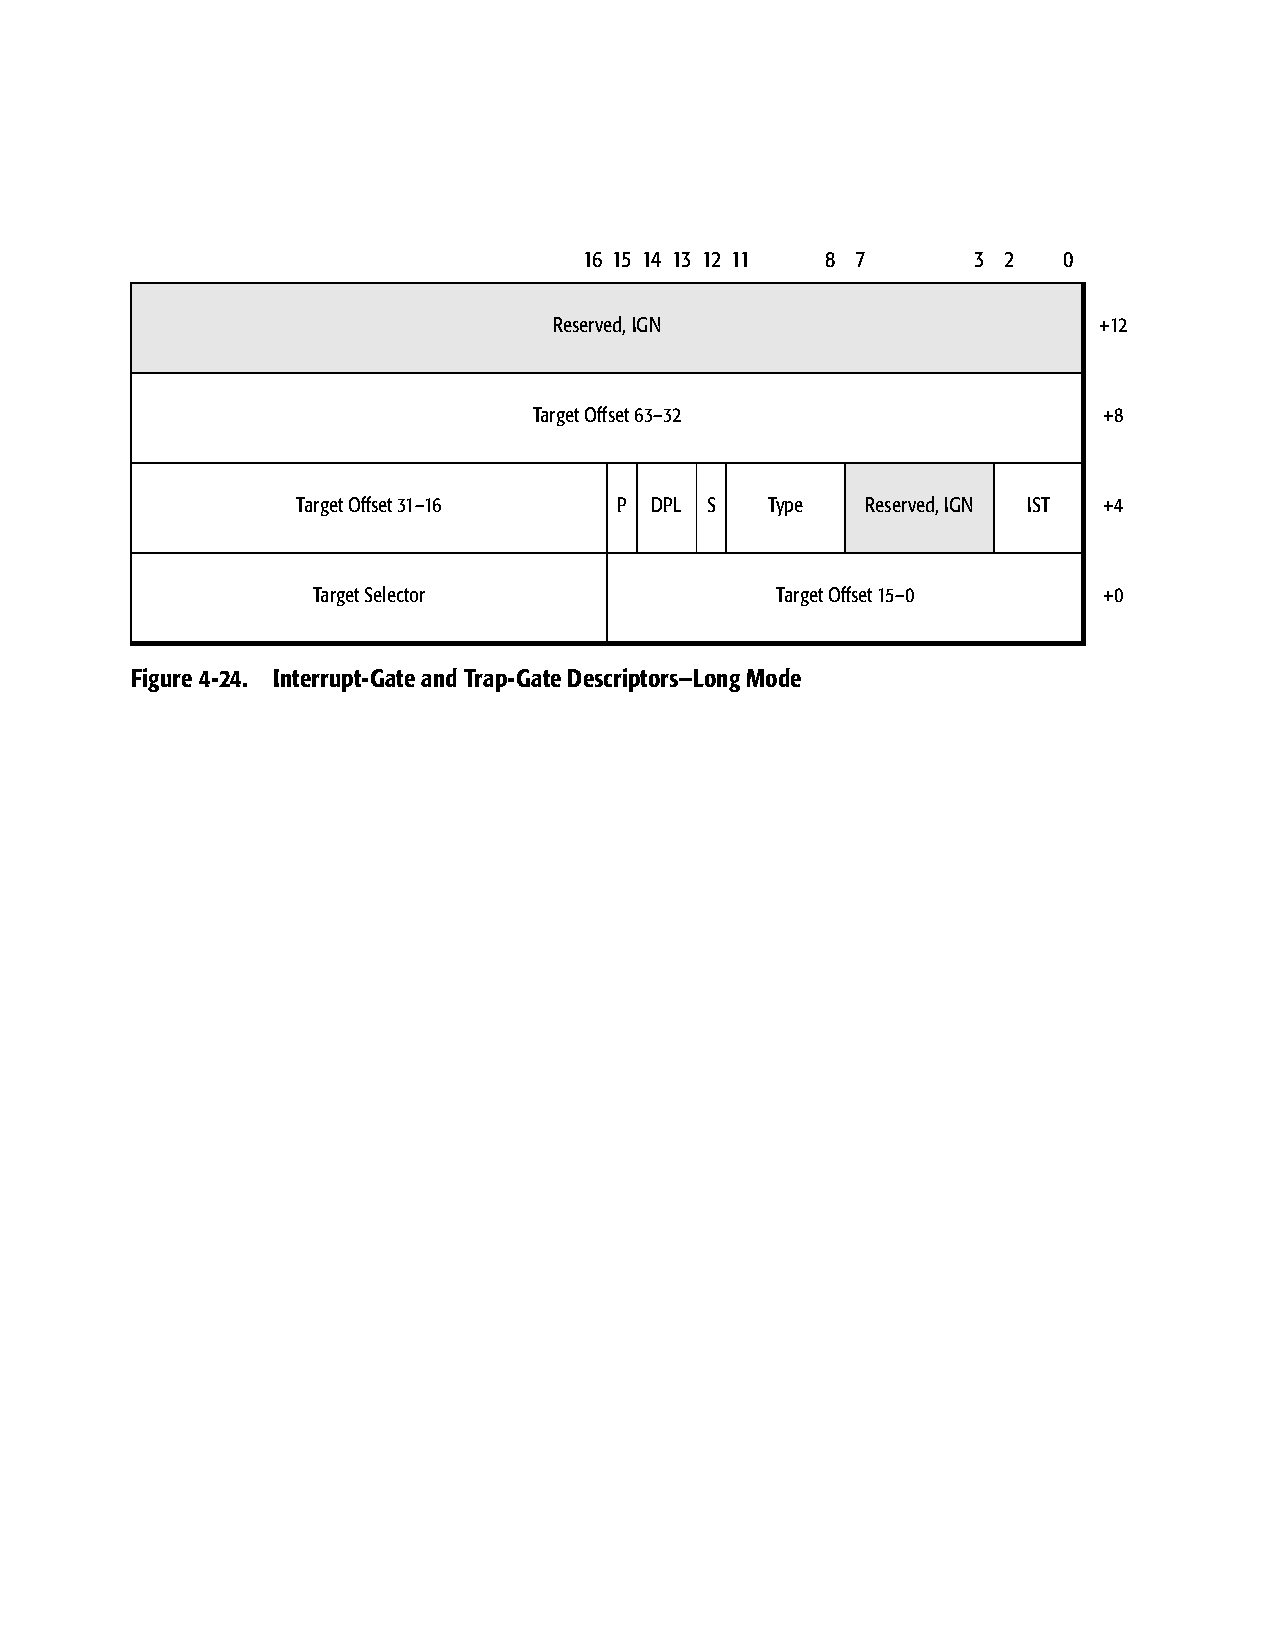
\includegraphics[height=30mm]{intgate.pdf}
}
\itms{
\item {\em Target Offset}: First instruction of the interrupt handler
\item {\em Target Selector}: Code segment -- sets privilege level (user/kernel 
    mode)
    \ittms{
    \item More on this later
    }
\item {\em P}: Present (i.e. valid)
\item {\em DPL}: Minimum privilege level that can trigger it
    \ittms{
    \item Prevents user programs from triggering device interrupts
    }
\item {\em Type}: Constant for 64-bit IDT entry
\item {\em IST}: Kernel stack to use
}
\end{slide}

\begin{slide}{Configuring Interrupt Handling (x86--64)}
\begin{enumerate}
\item OS initializes IDT with entry point of interrupt vectors (1-255)
\item OS initializes the IDT descriptor containing address and length of IDT
\item OS uses \code{lidt} instruction to load the IDTR
\end{enumerate}
\centerline{
    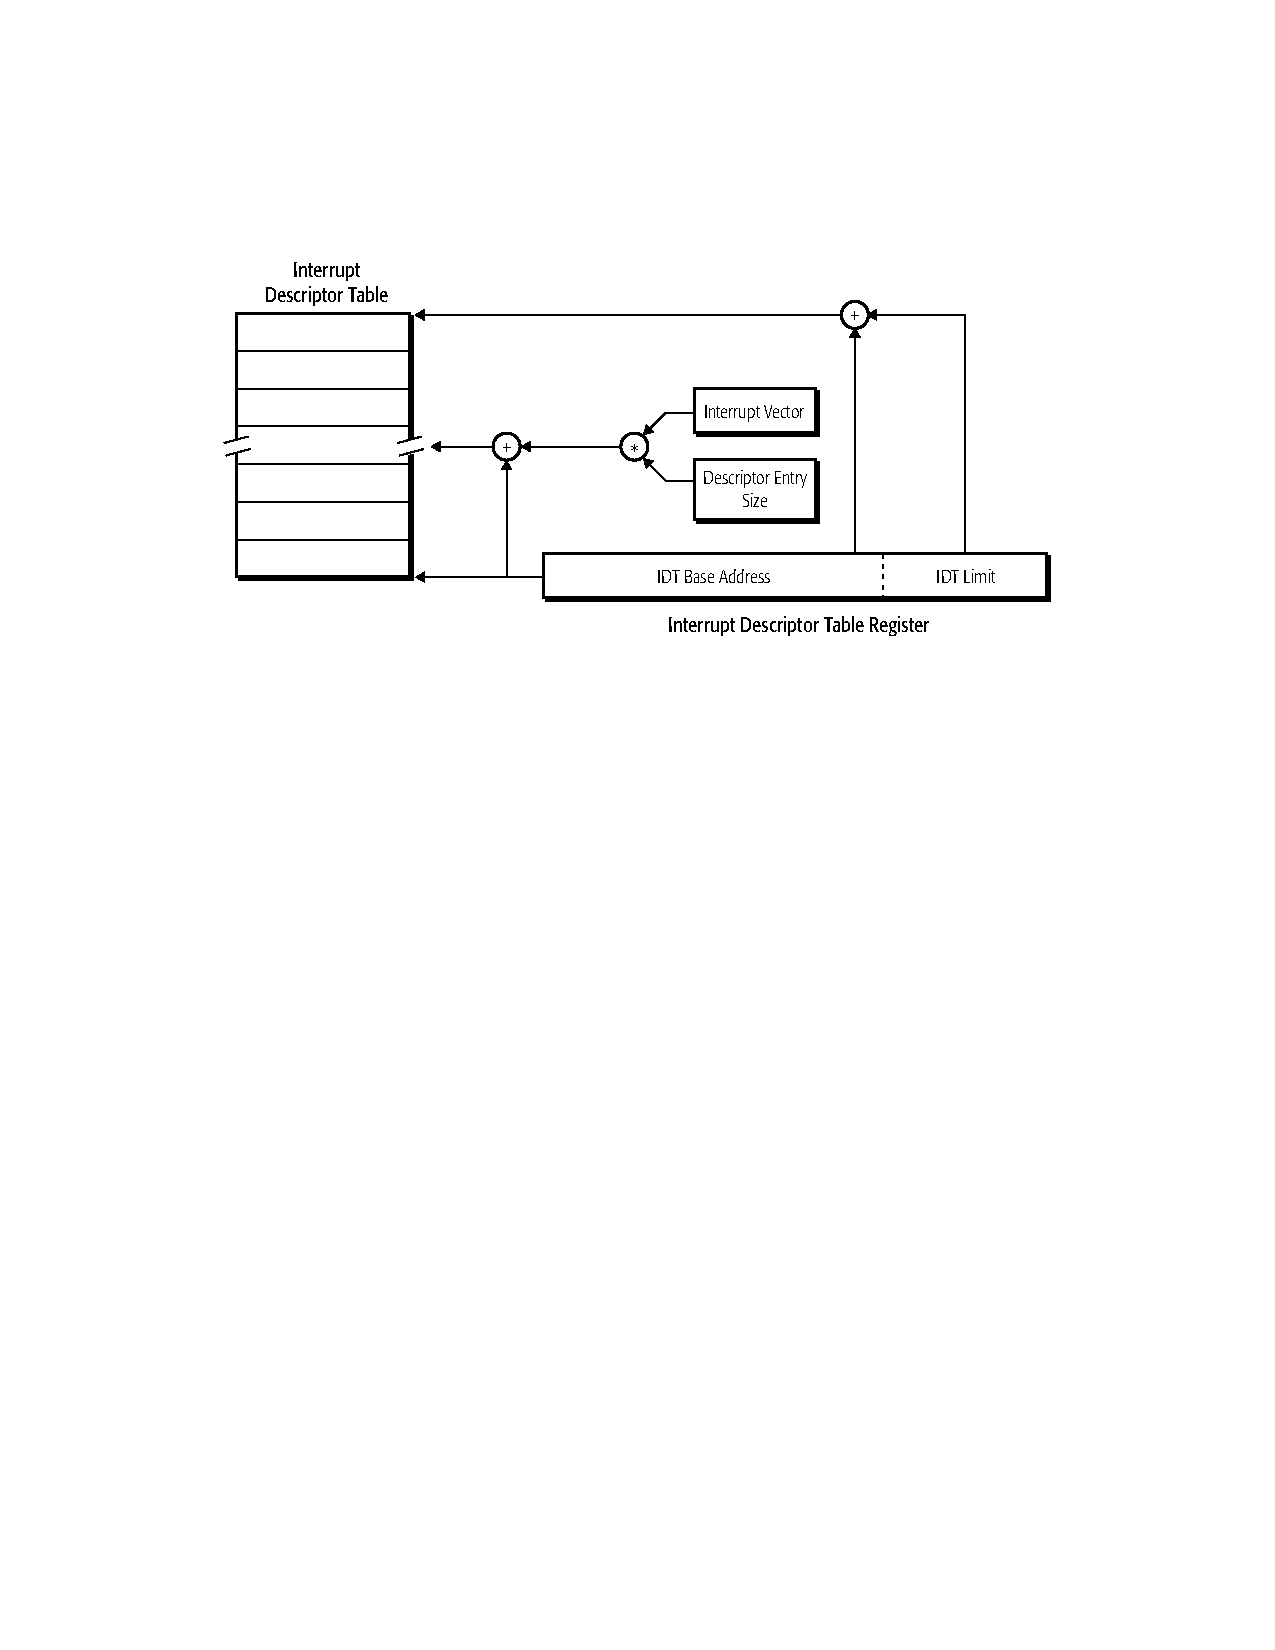
\includegraphics[height=55mm]{idtr.pdf}
}
\end{slide}

\begin{slide}{Hardware Interrupt Handling Process (x86--64)}
\begin{enumerate}
\item Finds the IDT through the IDTR register
\item Read the IDT descriptor entry
\item Look up the kernel stack in the TSS (Task State Segment)
\item IST field specifies which stack to use
\item CPU pushes the interrupt stack frame
\end{enumerate}
\centerline{
    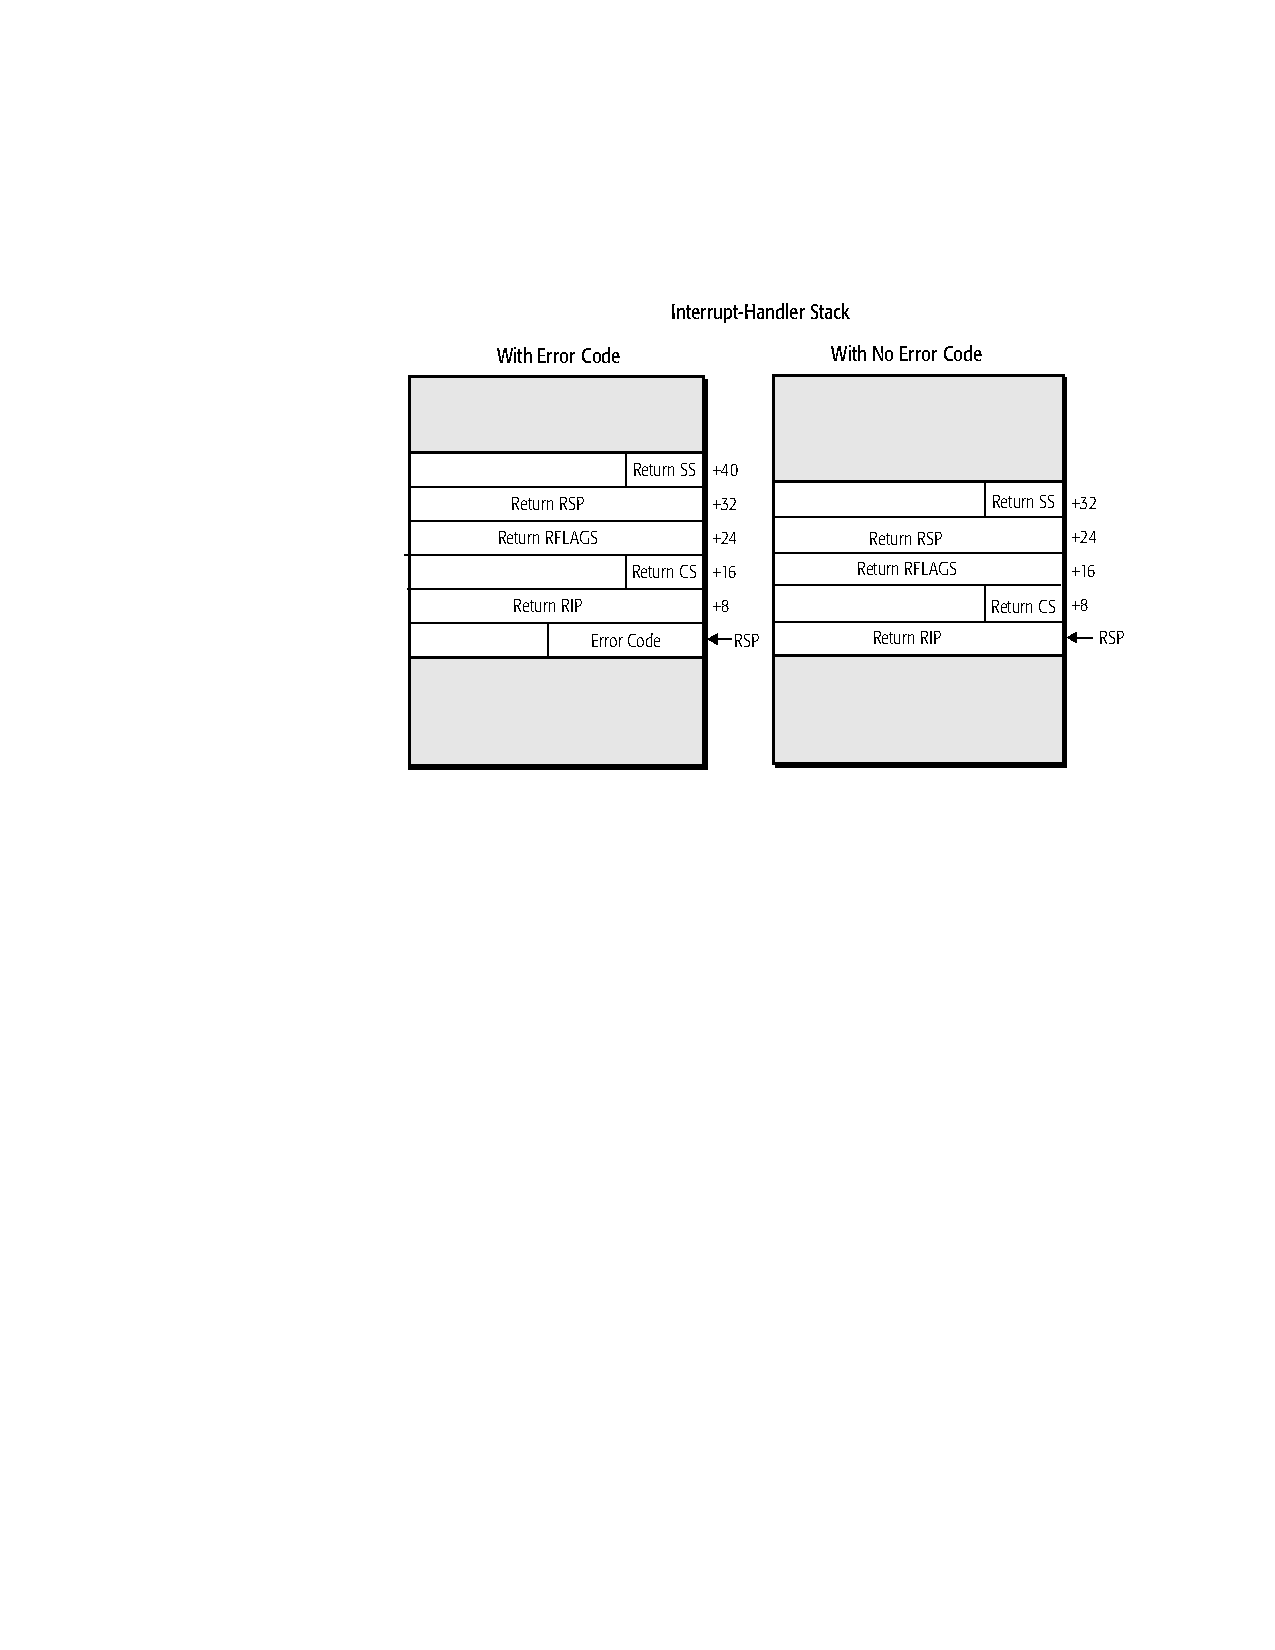
\includegraphics[height=45mm]{intstack.pdf}
}
\end{slide}

\begin{slide}{Hardware Interrupt Handling Process (x86--64)}
\begin{columns}
\column{0.6\textwidth}
\begin{enumerate}
\item Finds the IDT through the IDTR register
\item Read the IDT descriptor entry
\item Look up the kernel stack in the TSS (Task State Segment)
\item IST field specifies which stack to use
\item CPU pushes the interrupt stack frame
\item Kernel pushes the trap frame
\item Kernel sets up CPU to known state to run C code
\end{enumerate}
\column{0.4\textwidth}
\centerline{
    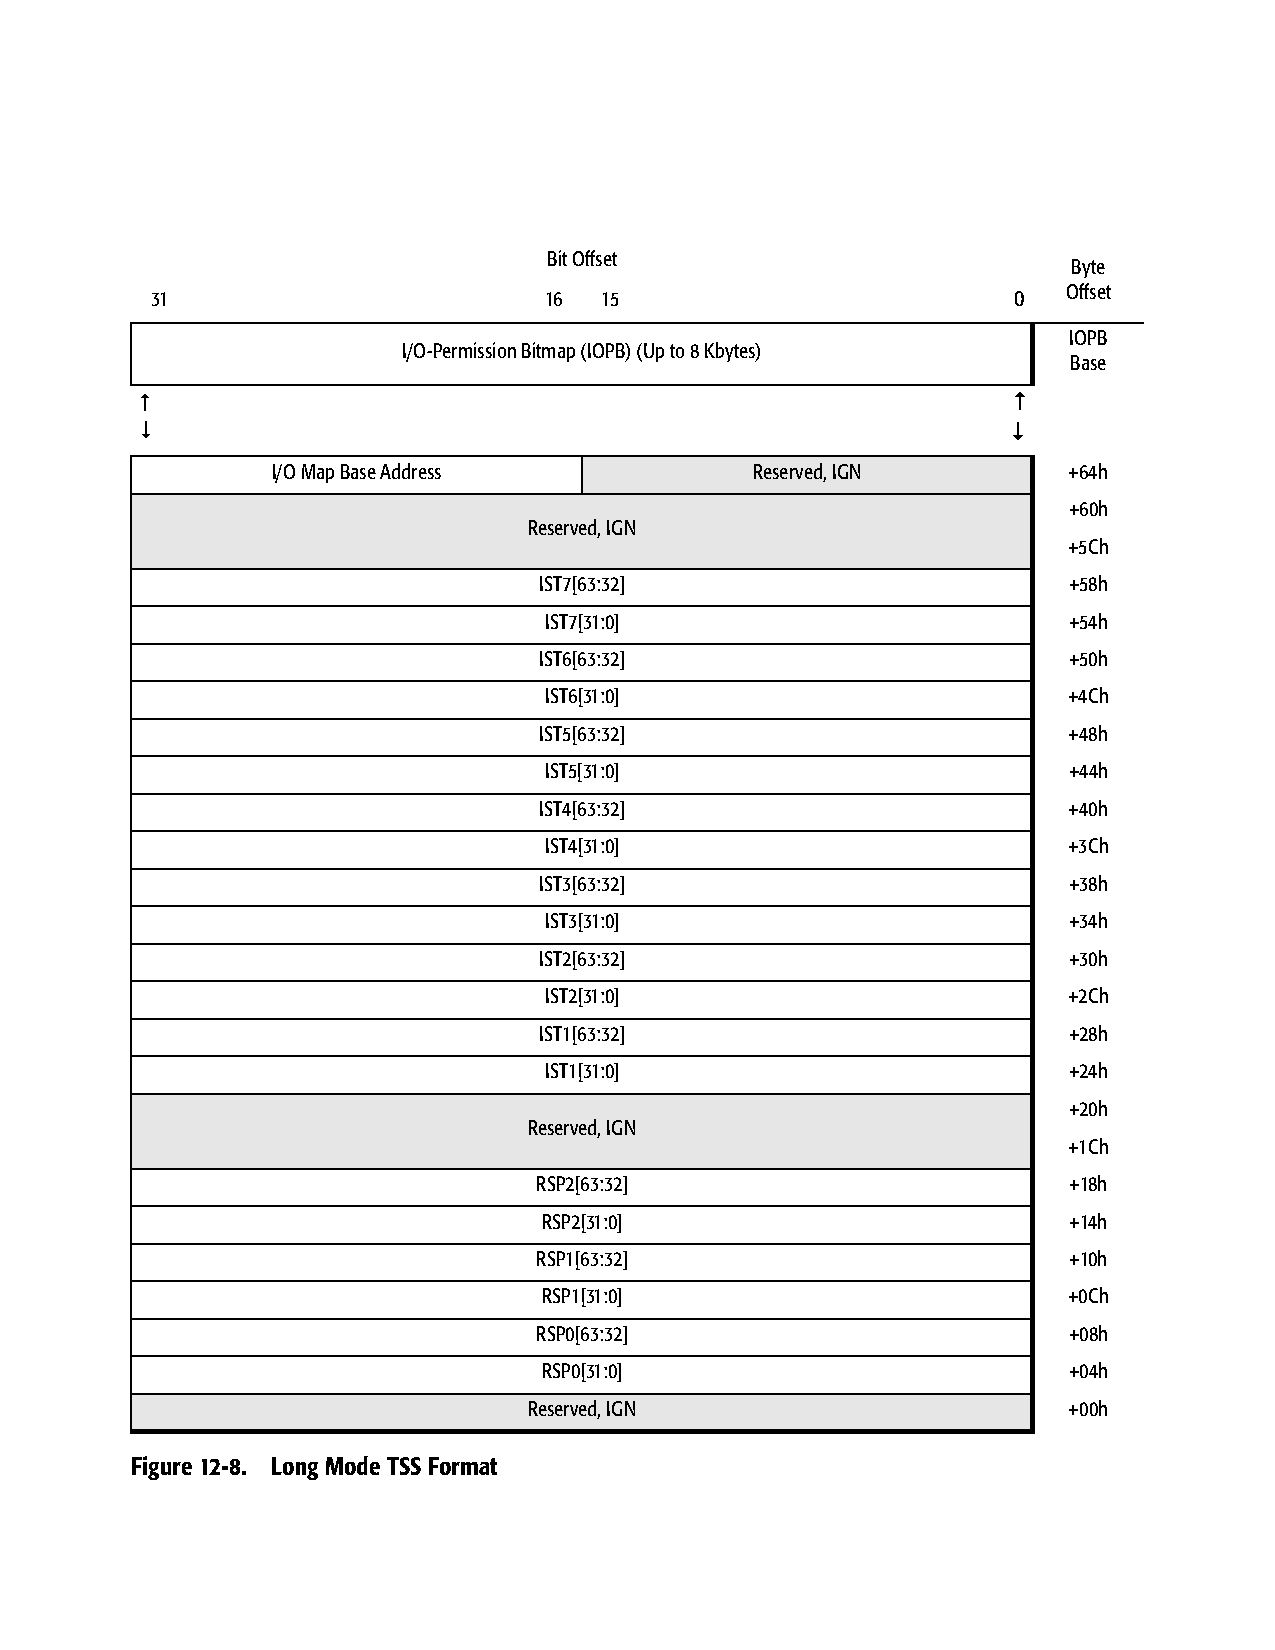
\includegraphics[height=75mm]{tss.pdf}
}
\end{columns}
\end{slide}

\begin{slide}{OS Handler Details}
\itms{
\item Interrupt Vectors defined in \grokdef{trap\_table}
\item IDT created and IDTR loaded in \grokdef{Trap\_Init}
\item Each interrupt vector has a custom assembly entry point
\item \grokdef{TRAP\_NOEC} and \grokdef{TRAP\_EC} macro for each
    \ittms{
    \item Pushes the start of the trap frame including vector number
    \item Most exceptions in x86 push an extra error code on the stack
    \item NOEC version pushes an extra 0 to make the stack layout identical
    }
\item \grokdef{trap\_common} pushes the CPU registers
\item \grokdef{trap\_entry} is the C handler that dispatches interrupts
}
\end{slide}

\begin{slide}{System Call Operation Details}
\itms{
\item Application calls into the C library (e.g., calls \texttt{write()})
\item Library executes the \texttt{syscall} instruction
\item Kernel exception handler runs
\ittms{
\item Switch to kernel stack
\item Create a {\em trapframe} which contains the program state
\item Determine the type of exception
\item Determine the type of system call
\item Run the function in the kernel (e.g., \texttt{sys\_write()})
\item Restore application state from the trap frame
\item Return from exception (\code{iret} instruction)
}
\item Library wrapper function returns to the application
}
\end{slide}

\section{Calling Conventions}

\begin{slide}{How are values passed?}
\begin{block}{}
{\em Application Binary Interface} (ABI) defines the contract between functions 
    an application and system calls.
\end{block}
\itms{
\item Operating Systems and Compilers must obey these rules referred to as the 
    {\em calling convention}
\item Defines
    \ittms{
    \item Meaning of registers during function calls and system calls
    \item Who's responsible to save registers
    \item Describes stack alignment rules
    }
}
\end{slide}

\begin{slide}{System Call Numbering}
\itms{
\item System calls numbers defined in kern/include/syscall.h
\item Syscall number is passed as the first argument into syscall
\gap
}
\begin{ccode}
#define SYSCALL_NULL		0x00
#define SYSCALL_TIME		0x01
#define SYSCALL_GETPID		0x02
#define SYSCALL_EXIT		0x03
#define SYSCALL_SPAWN		0x04
#define SYSCALL_WAIT		0x05

// Memory
#define SYSCALL_MMAP		0x08
#define SYSCALL_MUNMAP		0x09
#define SYSCALL_MPROTECT	0x0A
...
\end{ccode}
\end{slide}

\begin{slide}{x86--64 Calling Conventions}
\vspace{-1em}
\itms{
\item {\em Caller-saved registers} are saved before calling another function
	\ittms{
	\item \code{r10}, \code{r11}: Scratch registers
	\item \code{rdi}, \code{rsi}, \code{rdx}, \code{rcx}, \code{r8}, 
	    \code{r9}: Argument registers
	\item \code{rax}, \code{rdx}: Return values
	}
\item {\em Callee-saved registers} are saved inside the function
	\ittms{
	\item \code{rbx}, \code{r12}--\code{r15}: Saved registers
	}
\item {\em Stack registers}
	\ittms{
	\item \code{rsp}: Stack pointer
	\item \code{rbp}: Frame pointer (assuming -fno-omit-framepointer)
	}
\item Instructions:
\ittms{
\item \code{call}: Call function and save return address on stack
\item \code{ret}: Return from function
}
}
\end{slide}

\begin{slide}{Functions in x86--64}
\itms{
\item Functions are called with the \texttt{call} instruction
\item \code{call} pushes the return address to the stack and jumps to the 
    target
\gap
}
\begin{x64asm}
foo:
	push %rbp # Save the frame pointer
	mov %rsp, %rbp # Set the frame pointer to TOS

	# Save caller-save registers (if needed)

	call bar # Call bar

	# Restore registers (if needed)

	pop %rbp
	ret # Return
\end{x64asm}
\end{slide}

\begin{slide}{Functions in x86--64 Continued}
\itms{
\item Simple functions may not need to save any registers
\item We save callee-saved registers if needed for performance
\gap
}
\begin{ccode}
int bar(int a) {
	return 41 + a;
}
\end{ccode}

\begin{x64asm}
bar:
	mov %edi, %eax # Move 1st arg to eax (lower 32-bits of rax)
	add $41, %eax # Add 41 to eax
	ret
\end{x64asm}
\end{slide}

\begin{slide}{Where are registers saved?}
\vspace{-1em}
\begin{columns}
\column{0.7\textwidth}
\itms{
\item Registers are saved in memory in the per-thread stack
\item A \emph{stack frame} is all the saved registers and local variables that 
	must be saved within a single function
\item Our stack is made up of an array of stack frames
}
\gap
\begin{x64asm}
	# Push stack element
	push %rax
	# Equivalent to:
	mov %rax, -8(%rsp) # Store into the top of stack
	sub $8, %rsp

	# Pop stack element
	pop %rax
	# Equivalent to:
	mov 0(%rsp), %rax # Load from the top of stack
	add $8, %rsp
\end{x64asm}
\column{0.3\textwidth}
\end{columns}
\end{slide}

\section{System Calls}

\begin{slide}{Execution Contexts}
\begin{block}{}
{\em Execution Context}: The environment where functions execute including 
	their arguments, local variables, memory.
\end{block}
\itms{
\item Context is a unique set of CPU registers and a stack pointer
\gap
\item Multiple execution contexts:
\ittms{
\item {\em Application Context}: Application threads
\item {\em Kernel Context}: Kernel threads, software interrupts, etc
\item {\em Interrupt Context}: Interrupt handler
}
\item Kernel and Interrupts usually the same context
\gap
\item Context transitions:
\ittms{
\item {\em Context switch}: a transitions between contexts
\item {\em Thread Switch}: a transition between threads (usually between kernel 
    contexts)
}
}
\end{slide}

\pgfdeclarelayer{background}
\pgfdeclarelayer{foreground}
\pgfsetlayers{background,main,foreground}
\tikzstyle{stk}=[draw, fill=white, text width=12em, text centered, minimum 
height=14.75em]
\tikzstyle{sstk}=[draw, fill=white, text width=12em, text centered, minimum 
height=1.5em]
\tikzstyle{mstk}=[draw, fill=white, text width=12em, text centered, minimum 
height=4em]
\tikzstyle{lstk}=[draw, fill=white, text width=12em, text centered, minimum 
height=6em]
\tikzstyle{lbl}=[align=center]

\begin{frame}{Application Stack}
\vspace{-1em}
\itms{
	\item Stack made of up {\em frames} containing locals, arguments, and spilled registers
\item Programs begin execution at \texttt{\_start}
}
\begin{figure}
\begin{tikzpicture}
	\node (f0) [stk] {};
	\path (f0.north) node (f1) [sstk] {{\tt \_start} frame};
	\path (f0.south)+(0,-1em) node (lbl) {User Stack};
\end{tikzpicture}
\end{figure}
\end{frame}

\begin{frame}{Application Stack}
\vspace{-1em}
\itms{
	\item Stack made of up {\em frames} containing locals, arguments, and spilled registers
\item Programs begin execution at \code{_start}
}
\begin{figure}
\begin{tikzpicture}
	\node (f0) [stk] {};
	\path (f0.north) node (f1) [sstk] {{\tt \_start} frame};
	\path (f1)+(0,-1.5em) node (f2) [sstk] {{\tt main()} frame};
	\path (f0.south)+(0,-1em) node (lbl) {User Stack};
\end{tikzpicture}
\end{figure}
\end{frame}

\begin{frame}{Application Stack}
\vspace{-1em}
\itms{
\item Stack made of up {\em frames} containing locals, arguments, and spilled registers
\item Programs begin execution at \texttt{\_start}
}
\begin{figure}
\begin{tikzpicture}
	\node (f0) [stk] {};
	\path (f0.north) node (f1) [sstk] {{\tt \_start} frame};
	\path (f1)+(0,-1.5em) node (f2) [sstk] {{\tt main()} frame};
	\path (f2)+(0,-1.5em) node (f3) [sstk] {{\tt printf()} frame};
	\path (f0.south)+(0,-1em) node (lbl) {User Stack};
\end{tikzpicture}
\end{figure}
\end{frame}

\begin{frame}{Application Stack}
\vspace{-1em}
\itms{
\item Stack made of up {\em frames} containing locals, arguments, and spilled registers
\item Programs begin execution at \texttt{\_start}
}
\begin{figure}
\begin{tikzpicture}
	\node (f0) [stk] {};
	\path (f0.north) node (f1) [sstk] {{\tt \_start} frame};
	\path (f1)+(0,-1.5em) node (f2) [sstk] {{\tt main()} frame};
	\path (f2)+(0,-1.5em) node (f3) [sstk] {{\tt printf()} frame};
	\path (f3)+(0,-1.5em) node (f4) [sstk] {{\tt write()} frame};
	\path (f0.south)+(0,-1em) node (lbl) {User Stack};
\end{tikzpicture}
\end{figure}
\end{frame}

\begin{frame}{Application Stack}
\vspace{-1em}
\itms{
\item Stack made of up {\em frames} containing locals, arguments, and spilled registers
\item Programs begin execution at \texttt{\_start}
}
\begin{figure}
\begin{tikzpicture}
	\node (f0) [stk] {};
	\path (f0.north) node (f1) [sstk] {{\tt \_start} frame};
	\path (f1)+(0,-1.5em) node (f2) [sstk] {{\tt main()} frame};
	\path (f2)+(0,-1.5em) node (f3) [sstk] {{\tt printf()} frame};
	\path (f3)+(0,-1.5em) node (f4) [sstk] {{\tt write()} frame};
	\path (f4)+(0,-2.75em) node (f5) [mstk] {???};
	\path (f0.south)+(0,-1em) node (lbl) {User Stack};
\end{tikzpicture}
\end{figure}
\end{frame}

\begin{frame}{Context Switch: User to Kernel}
\vspace{-1em}
\itms{
\item {\em trapframe}: Saves the application context
\item \code{int $60} instruction triggers the exception handler (vector 60)
}
\begin{figure}
\begin{tikzpicture}
	\node (f0) [stk] {};
	\path (f0.north) node (f1) [sstk] {{\tt \_start} frame};
	\path (f1)+(0,-1.5em) node (f2) [sstk] {{\tt main()} frame};
	\path (f2)+(0,-1.5em) node (f3) [sstk] {{\tt printf()} frame};
	\path (f3)+(0,-1.5em) node (f4) [sstk] {{\tt write()} frame};
	\path (f0.south)+(0,-1em) node (lbl) {User Stack};

	\path (f0)+(14em,0) node (k0) [stk] {};
	\path (k0.north)+(0,-1.25em) node (k1) [mstk]
	{{\tt trap\_common}\\trapframe};
	\path (k0.south)+(0,-1em) node (lbl) {Kernel Stack};
\end{tikzpicture}
\end{figure}
\end{frame}

\begin{frame}{Context Switch: User to Kernel}
\vspace{-1em}
\itms{
\item {\em trapframe}: Saves the application context
\item \code{trap_common} saves trapframe on the kernel stack!
}
\begin{figure}
\begin{tikzpicture}
	\node (f0) [stk] {};
	\path (f0.north) node (f1) [sstk] {{\tt \_start} frame};
	\path (f1)+(0,-1.5em) node (f2) [sstk] {{\tt main()} frame};
	\path (f2)+(0,-1.5em) node (f3) [sstk] {{\tt printf()} frame};
	\path (f3)+(0,-1.5em) node (f4) [sstk] {{\tt write()} frame};
	\path (f0.south)+(0,-1em) node (lbl) {User Stack};

	\path (f0)+(14em,0) node (k0) [stk] {};
	\path (k0.north)+(0,-1.25em) node (k1) [mstk]
	{{\tt trap\_common}\\{\em trapframe}};
	\path (k1)+(0,-2.75em) node (k2) [sstk] {\tt trap\_entry()};
	\path (k0.south)+(0,-1em) node (lbl) {Kernel Stack};
\end{tikzpicture}
\end{figure}
\end{frame}

\begin{frame}{Context Switch: User to Kernel}
\vspace{-1em}
\itms{
\item {\em trapframe}: Saves the application context
\item Calls \code{trap_entry()} to decode trap and \code{Syscall_Entry()}
}
\begin{figure}
\begin{tikzpicture}
	\node (f0) [stk] {};
	\path (f0.north) node (f1) [sstk] {{\tt \_start} frame};
	\path (f1)+(0,-1.5em) node (f2) [sstk] {{\tt main()} frame};
	\path (f2)+(0,-1.5em) node (f3) [sstk] {{\tt printf()} frame};
	\path (f3)+(0,-1.5em) node (f4) [sstk] {{\tt write()} frame};
	\path (f0.south)+(0,-1em) node (lbl) {User Stack};

	\path (f0)+(14em,0) node (k0) [stk] {};
	\path (k0.north)+(0,-1.25em) node (k1) [mstk]
	{{\tt trap\_common}\\{\em trapframe}};
	\path (k1)+(0,-2.75em) node (k2) [sstk] {\tt trap\_entry()};
	\path (k2)+(0,-1.5em) node (k3) [sstk] {\tt Syscall\_Entry()};
	\path (k0.south)+(0,-1em) node (lbl) {Kernel Stack};
\end{tikzpicture}
\end{figure}
\end{frame}

\begin{frame}{Context Switch: User to Kernel}
\vspace{-1em}
\itms{
\item {\em trapframe}: Saves the application context
\item \code{Syscall_Entry()} decodes arguments and calls \code{Syscall_Write()}
}
\begin{figure}
\begin{tikzpicture}
	\node (f0) [stk] {};
	\path (f0.north) node (f1) [sstk] {{\tt \_start} frame};
	\path (f1)+(0,-1.5em) node (f2) [sstk] {{\tt main()} frame};
	\path (f2)+(0,-1.5em) node (f3) [sstk] {{\tt printf()} frame};
	\path (f3)+(0,-1.5em) node (f4) [sstk] {{\tt write()} frame};
	\path (f0.south)+(0,-1em) node (lbl) {User Stack};

	\path (f0)+(14em,0) node (k0) [stk] {};
	\path (k0.north)+(0,-1.25em) node (k1) [mstk]
	{{\tt trap\_common}\\{\em trapframe}};
	\path (k1)+(0,-2.75em) node (k2) [sstk] {\tt trap\_entry()};
	\path (k2)+(0,-1.5em) node (k3) [sstk] {\tt Syscall\_Entry()};
	\path (k3)+(0,-1.5em) node (k4) [sstk] {\tt Syscall\_Write()};
	\path (k0.south)+(0,-1em) node (lbl) {Kernel Stack};
\end{tikzpicture}
\end{figure}
\end{frame}

\begin{frame}{Context Switch: Returning to User Mode}
\vspace{-1em}
\itms{
\item {\em trapframe}: Saves the application context
\item \code{Syscall_Write()} writes text to console
}
\begin{figure}
\begin{tikzpicture}
	\node (f0) [stk] {};
	\path (f0.north) node (f1) [sstk] {{\tt \_start} frame};
	\path (f1)+(0,-1.5em) node (f2) [sstk] {{\tt main()} frame};
	\path (f2)+(0,-1.5em) node (f3) [sstk] {{\tt printf()} frame};
	\path (f3)+(0,-1.5em) node (f4) [sstk] {{\tt write()} frame};
	\path (f0.south)+(0,-1em) node (lbl) {User Stack};

	\path (f0)+(14em,0) node (k0) [stk] {};
	\path (k0.north)+(0,-1.25em) node (k1) [mstk]
	{{\tt trap\_common}\\{\em trapframe}};
	\path (k1)+(0,-2.75em) node (k2) [sstk] {\tt trap\_entry()};
	\path (k2)+(0,-1.5em) node (k3) [sstk] {\tt Syscall\_Entry()};
	\path (k3)+(0,-1.5em) node (k4) [sstk] {\tt Syscall\_Write()};
	\path (k4)+(0,-2.75em) node (k5) [mstk] {\em console\\driver};
	\path (k0.south)+(0,-1em) node (lbl) {Kernel Stack};
\end{tikzpicture}
\end{figure}
\end{frame}

\begin{frame}{Context Switch: Returning to User Mode}
\vspace{-1em}
\itms{
\item {\em trapframe}: Saves the application context
\item Return from \code{Syscall_Write()}
}
\begin{figure}
\begin{tikzpicture}
	\node (f0) [stk] {};
	\path (f0.north) node (f1) [sstk] {{\tt \_start} frame};
	\path (f1)+(0,-1.5em) node (f2) [sstk] {{\tt main()} frame};
	\path (f2)+(0,-1.5em) node (f3) [sstk] {{\tt printf()} frame};
	\path (f3)+(0,-1.5em) node (f4) [sstk] {{\tt write()} frame};
	\path (f0.south)+(0,-1em) node (lbl) {User Stack};

	\path (f0)+(14em,0) node (k0) [stk] {};
	\path (k0.north)+(0,-1.25em) node (k1) [mstk]
	{{\tt trap\_common}\\{\em trapframe}};
	\path (k1)+(0,-2.75em) node (k2) [sstk] {\tt trap\_entry()};
	\path (k2)+(0,-1.5em) node (k3) [sstk] {\tt Syscall\_Entry()};
	\path (k3)+(0,-1.5em) node (k4) [sstk] {\tt Syscall\_Write()};
	\path (k0.south)+(0,-1em) node (lbl) {Kernel Stack};
\end{tikzpicture}
\end{figure}
\end{frame}

\begin{frame}{Context Switch: Returning to User Mode}
\vspace{-1em}
\itms{
\item \code{Syscall_Entry()} stores return value and error in trapframe
\item {\tt rax}: return value/error code
}
\begin{figure}
\begin{tikzpicture}
	\node (f0) [stk] {};
	\path (f0.north) node (f1) [sstk] {{\tt \_start} frame};
	\path (f1)+(0,-1.5em) node (f2) [sstk] {{\tt main()} frame};
	\path (f2)+(0,-1.5em) node (f3) [sstk] {{\tt printf()} frame};
	\path (f3)+(0,-1.5em) node (f4) [sstk] {{\tt write()} frame};
	\path (f0.south)+(0,-1em) node (lbl) {User Stack};

	\path (f0)+(14em,0) node (k0) [stk] {};
	\path (k0.north)+(0,-1.25em) node (k1) [mstk]
	{{\tt trap\_common}\\{\em trapframe}};
	\path (k1)+(0,-2.75em) node (k2) [sstk] {\tt trap\_entry()};
	\path (k2)+(0,-1.5em) node (k3) [sstk] {\tt Syscall\_Entry()};
	\path (k0.south)+(0,-1em) node (lbl) {Kernel Stack};
\end{tikzpicture}
\end{figure}
\end{frame}

\begin{frame}{Context Switch: Returning to User Mode}
\vspace{-1em}
\itms{
\item \code{trap_common()} returns to the instruction following \code{int $60}
\item {\tt rax}: return value/error code
}
\begin{figure}
\begin{tikzpicture}
	\node (f0) [stk] {};
	\path (f0.north) node (f1) [sstk] {{\tt \_start} frame};
	\path (f1)+(0,-1.5em) node (f2) [sstk] {{\tt main()} frame};
	\path (f2)+(0,-1.5em) node (f3) [sstk] {{\tt printf()} frame};
	\path (f3)+(0,-1.5em) node (f4) [sstk] {{\tt write()} frame};
	\path (f0.south)+(0,-1em) node (lbl) {User Stack};

	\path (f0)+(14em,0) node (k0) [stk] {};
	\path (k0.north)+(0,-1.25em) node (k1) [mstk]
	{{\tt trap\_common}\\{\em trapframe}};
	\path (k1)+(0,-2.75em) node (k2) [sstk] {\tt trap\_entry()};
	\path (k0.south)+(0,-1em) node (lbl) {Kernel Stack};
\end{tikzpicture}
\end{figure}
\end{frame}

\begin{frame}{Context Switch: Returning to User Mode}
	\vspace{-1em}
\itms{
\item {\tt trap\_common} restores the application context
\item Restores all CPU state from the trapframe
}
\begin{figure}
\begin{tikzpicture}
	\node (f0) [stk] {};
	\path (f0.north) node (f1) [sstk] {{\tt \_start} frame};
	\path (f1)+(0,-1.5em) node (f2) [sstk] {{\tt main()} frame};
	\path (f2)+(0,-1.5em) node (f3) [sstk] {{\tt printf()} frame};
	\path (f3)+(0,-1.5em) node (f4) [sstk] {{\tt write()} frame};
	\path (f0.south)+(0,-1em) node (lbl) {User Stack};

	\path (f0)+(14em,0) node (k0) [stk] {};
	\path (k0.north)+(0,-1.25em) node (k1) [mstk]
	{{\tt trap\_common}\\{\em trapframe}};
	\path (k0.south)+(0,-1em) node (lbl) {Kernel Stack};
\end{tikzpicture}
\end{figure}
\end{frame}

\begin{frame}{Context Switch: Returning to User Mode}
	\vspace{-1em}
\itms{
\item {\tt write()} decodes {\tt rax} and updates {\tt errno}
\item {\em errno} is where error codes are stored in POSIX
}
\begin{figure}
\begin{tikzpicture}
	\node (f0) [stk] {};
	\path (f0.north) node (f1) [sstk] {{\tt \_start} frame};
	\path (f1)+(0,-1.5em) node (f2) [sstk] {{\tt main()} frame};
	\path (f2)+(0,-1.5em) node (f3) [sstk] {{\tt printf()} frame};
	\path (f3)+(0,-1.5em) node (f4) [sstk] {{\tt write()} frame};
	\path (f0.south)+(0,-1em) node (lbl) {User Stack};

	\path (f0)+(14em,0) node (k0) [stk] {};
	\path (k0.south)+(0,-1em) node (lbl) {Kernel Stack};
\end{tikzpicture}
\end{figure}
\end{frame}

\begin{frame}{Context Switch: Returning to User Mode}
\vspace{-1em}
\itms{
\item {\em errno} is where error codes are stored in POSIX
\item {\tt printf()} gets return value, if -1 then sets {\tt errno}
}
\begin{figure}
\begin{tikzpicture}
	\node (f0) [stk] {};
	\path (f0.north) node (f1) [sstk] {{\tt \_start} frame};
	\path (f1)+(0,-1.5em) node (f2) [sstk] {{\tt main()} frame};
	\path (f2)+(0,-1.5em) node (f3) [sstk] {{\tt printf()} frame};
	\path (f0.south)+(0,-1em) node (lbl) {User Stack};

	\path (f0)+(14em,0) node (k0) [stk] {};
	\path (k0.south)+(0,-1em) node (lbl) {Kernel Stack};
\end{tikzpicture}
\end{figure}
\end{frame}

\section{Switching Threads/Processes}

\begin{slide}{Scheduling}
\itms{
\item How to pick which process to run
\item Scan process table for first runnable?
\ittms{
  \item Expensive.  Weird priorities (small pids do better)
  \item Divide into runnable and blocked processes
}
\item FIFO/Round-Robin?
\ittms{
  \item Put threads on back of list, pull them from front \\
  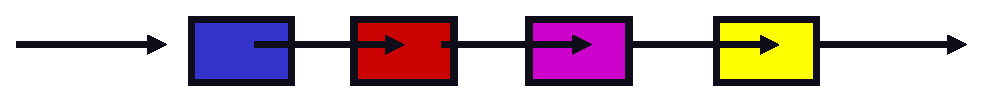
\includegraphics[width=2.5in]{figs/proclist} \\
  (see \texttt{kern/sched.c})
}
\item Priority?
\ittms{
  \item Give some threads a better shot at the CPU
}
}
\end{slide}

\begin{slide}{Preemption}
\itms{
  \item Can preempt a process when kernel gets control
  \item Running process can vector control to kernel
  \ittms{
    \item System call, page fault, illegal instruction, etc.
    \item May put current process to sleep---e.g., read from disk
    \item May make other process runnable---e.g., fork, write to pipe
  }
  \item Periodic timer interrupt
  \ittms{
    \item If running process used up quantum, schedule another
  }
  \item Device interrupt
  \ittms{
    \item Disk request completed, or packet arrived on network
    \item Previously waiting process becomes runnable
    \item Schedule if higher priority than current running proc.
  }
  \item Changing running process is called a \emph{context switch}
}
\end{slide}

\begin{slide}{Context switch}
\centerline{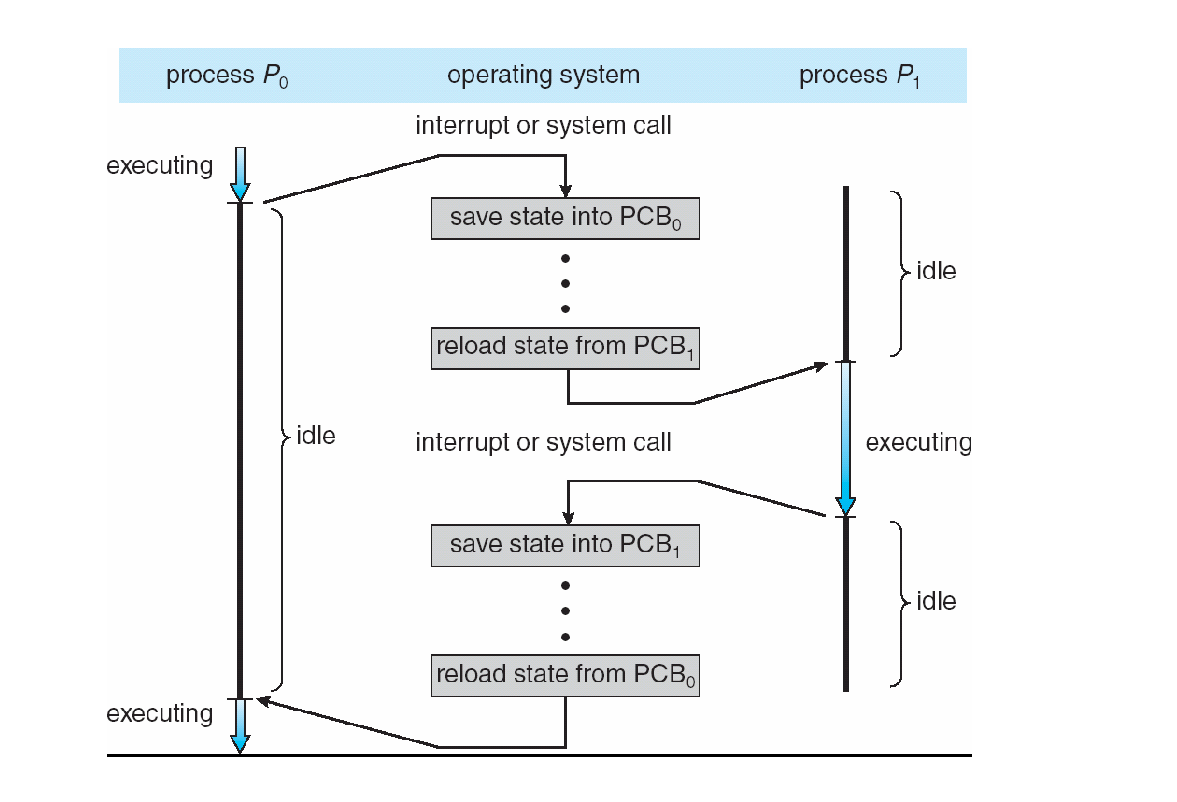
\includegraphics[height=70mm]{figs/switch}}
\end{slide}

\begin{slide}{Context switch details}
\itms{
  \item Very machine dependent.  Typical things include:
  \ittms{
    \item Save program counter and integer registers (always)
    \item Save floating point or other special registers
    \item Save condition codes
    \item Change virtual address translations
  }
  \gap
  \item Non-negligible cost
  \ittms{
    \item Save/restore floating point registers expensive \\
    \itttms{
      \item Optimization: only save if process used floating point
    }
    \item May require flushing TLB (memory translation hardware) \\
    \itttms{
      \item HW Optimization~1: don't flush kernel's own data from TLB
      \item HW Optimization~2: use tag to avoid flushing any data
    }
    \item Usually causes more cache misses (switch working sets)
  }
}
\end{slide}

\begin{frame}{Switching Processes: Timer Interrupt}
\vspace{-1em}
\itms{
\item Starts with a timer interrupt or sleeping in a system call
\item Interrupts user process in the middle of the execution

}
\begin{figure}
\begin{tikzpicture}
	\node (f0) [stk] {};
	\path (f0.north) node (f1) [sstk] {{\tt \_start} frame};
	\path (f1)+(0,-1.5em) node (f2) [sstk] {{\tt main()} frame};
	\path (f0.south)+(0,-1em) node (lbl) {User Stack};

	\path (f0)+(14em,0) node (k0) [stk] {};
	\path (k0.north)+(0,-1.25em) node (k1) [mstk]
	{{\tt trap\_common}\\{\em trapframe}};
	\path (k0.south)+(0,-1em) node (lbl) {Kernel Stack 1};
\end{tikzpicture}
\end{figure}
\end{frame}

\begin{frame}{Switching Processes: Timer Interrupt}
\vspace{-1em}
\itms{
\item \code{trap_common} saves the trapframe
\item \code{Trap_Entry()} notices a \code{T_IRQ_TIMER} from the Timer

}
\begin{figure}
\begin{tikzpicture}
	\node (f0) [stk] {};
	\path (f0.north) node (f1) [sstk] {{\tt \_start} frame};
	\path (f1)+(0,-1.5em) node (f2) [sstk] {{\tt main()} frame};
	\path (f0.south)+(0,-1em) node (lbl) {User Stack};

	\path (f0)+(14em,0) node (k0) [stk] {};
	\path (k0.north)+(0,-1.25em) node (k1) [mstk]
	{{\tt trap\_common}\\{\em trapframe}};
	\path (k1)+(0,-2.75em) node (k2) [sstk] {\tt Trap\_Entry()};
	\path (k0.south)+(0,-1em) node (lbl) {Kernel Stack 1};
\end{tikzpicture}
\end{figure}
\end{frame}

\begin{frame}{Switching Processes: Timer Interrupt}
\vspace{-1em}
\itms{
\item Calls \code{KTimer_Process} to process any scheduled timer events
}
\begin{figure}
\begin{tikzpicture}
	\node (f0) [stk] {};
	\path (f0.north) node (f1) [sstk] {{\tt \_start} frame};
	\path (f1)+(0,-1.5em) node (f2) [sstk] {{\tt main()} frame};
	\path (f0.south)+(0,-1em) node (lbl) {User Stack};

	\path (f0)+(14em,0) node (k0) [stk] {};
	\path (k0.north)+(0,-1.25em) node (k1) [mstk]
	{{\tt trap\_common}\\{\em trapframe}};
	\path (k1)+(0,-2.75em) node (k2) [sstk] {\tt Trap\_Entry()};
	\path (k2)+(0,-1.5em) node (k3) [sstk] {\tt KTimer\_Process};
	\path (k0.south)+(0,-1em) node (lbl) {Kernel Stack 1};
\end{tikzpicture}
\end{figure}
\end{frame}

\begin{frame}{Switching Processes: Timer Interrupt}
\vspace{-1em}
\itms{
\item Calls \code{Sched_Scheduler} to switch to a new process
}
\begin{figure}
\begin{tikzpicture}
	\node (f0) [stk] {};
	\path (f0.north) node (f1) [sstk] {{\tt \_start} frame};
	\path (f1)+(0,-1.5em) node (f2) [sstk] {{\tt main()} frame};
	\path (f0.south)+(0,-1em) node (lbl) {User Stack};

	\path (f0)+(14em,0) node (k0) [stk] {};
	\path (k0.north)+(0,-1.25em) node (k1) [mstk]
	{{\tt trap\_common}\\{\em trapframe}};
	\path (k1)+(0,-2.75em) node (k2) [sstk] {\tt Trap\_Entry()};
	\path (k2)+(0,-1.5em) node (k3) [sstk] {\tt Sched\_Scheduler};
	\path (k0.south)+(0,-1em) node (lbl) {Kernel Stack 1};
\end{tikzpicture}
\end{figure}
\end{frame}


\begin{frame}{Switching Processes: Timer Interrupt}
\vspace{-1em}
\itms{
\item Timers trigger processing events in the OS and the CPU scheduler
}
\begin{figure}
\begin{tikzpicture}
	\node (f0) [stk] {};
	\path (f0.north) node (f1) [sstk] {{\tt \_start} frame};
	\path (f1)+(0,-1.5em) node (f2) [sstk] {{\tt main()} frame};
	\path (f0.south)+(0,-1em) node (lbl) {User Stack};

	\path (f0)+(14em,0) node (k0) [stk] {};
	\path (k0.north)+(0,-1.25em) node (k1) [mstk]
	{{\tt trap\_common}\\{\em trapframe}};
	\path (k1)+(0,-2.75em) node (k2) [sstk] {\tt Trap\_Entry()};
	\path (k2)+(0,-1.5em) node (k3) [sstk] {\tt Sched\_Scheduler};
	\path (k0.south)+(0,-1em) node (lbl) {Kernel Stack 1};
\end{tikzpicture}
\end{figure}
\end{frame}

\begin{frame}{Switching Processes: CPU Scheduler}
\vspace{-1em}
\itms{
\item \code{Sched_Scheduler()} calls into scheduler to pick next thread
\item Calls \code{Sched_Switch()} to switch threads
}
\begin{figure}
\begin{tikzpicture}
	\node (f0) [stk] {};
	\path (f0.north) node (f1) [sstk] {{\tt \_start} frame};
	\path (f1)+(0,-1.5em) node (f2) [sstk] {{\tt main()} frame};
	\path (f0.south)+(0,-1em) node (lbl) {User Stack};

	\path (f0)+(14em,0) node (k0) [stk] {};
	\path (k0.north)+(0,-1.25em) node (k1) [mstk]
	{{\tt trap\_common}\\{\em trapframe}};
	\path (k1)+(0,-2.75em) node (k2) [sstk] {\tt Trap\_Entry()};
	\path (k2)+(0,-1.5em) node (k3) [sstk] {\tt Sched\_Scheduler};
	\path (k3)+(0,-1.5em) node (k4) [sstk] {\tt Sched\_Switch};
	\path (k4)+(0,-1.5em) node (k5) [sstk] {\tt Sched\_SwitchArch};
	\path (k0.south)+(0,-1em) node (lbl) {Kernel Stack 1};
\end{tikzpicture}
\end{figure}
\end{frame}

\begin{frame}{Switching Processes: Thread Switch}
\vspace{-1em}
\itms{
\item \code{switchstack}: saves and restores kernel thread state
\item Switching processes is a switch between kernel threads!
}
\begin{figure}
\begin{tikzpicture}
	\node (f0) [stk] {};
	\path (f0.north) node (f1) [sstk] {{\tt \_start} frame};
	\path (f1)+(0,-1.5em) node (f2) [sstk] {{\tt main()} frame};
	\path (f0.south)+(0,-1em) node (lbl) {User Stack};

	\path (f0)+(14em,0) node (k0) [stk] {};
	\path (k0.north)+(0,-1.25em) node (k1) [mstk]
	{{\tt trap\_common}\\{\em trapframe}};
	\path (k1)+(0,-2.75em) node (k2) [sstk] {\tt Trap\_Entry()};
	\path (k2)+(0,-1.5em) node (k3) [sstk] {\tt Sched\_Scheduler};
	\path (k3)+(0,-1.5em) node (k4) [sstk] {\tt Sched\_Switch};
	\path (k4)+(0,-1.5em) node (k5) [sstk] {\tt Thread\_SwitchArch};
	\path (k5)+(0,-1.5em) node (k6) [sstk] {\tt switchstack};
	\path (k6)+(0,-2.75em) node (k7) [mstk] {\em switchframe};
	\path (k0.south)+(0,-1em) node (lbl) {Kernel Stack 1};
\end{tikzpicture}
\end{figure}
\end{frame}

\begin{frame}{Switching Processes: Thread Switch}
\vspace{-1em}
\itms{
\item {\tt switchstack} saves thread state onto the stack
\item {\em switchframe}: contains the kernel context!
}
\begin{figure}
\begin{tikzpicture}
	\node (k0) [stk] {};
	\path (k0.north)+(0,-1.25em) node (k1) [mstk]
	{{\tt trap\_common}\\{\em trapframe}};
	\path (k1)+(0,-2.75em) node (k2) [sstk] {\tt Trap\_Entry()};
	\path (k2)+(0,-1.5em) node (k3) [sstk] {\tt Sched\_Scheduler};
	\path (k3)+(0,-1.5em) node (k4) [sstk] {\tt Sched\_Switch};
	\path (k4)+(0,-1.5em) node (k5) [sstk] {\tt Thread\_SwitchArch};
	\path (k5)+(0,-1.5em) node (k6) [sstk] {\tt switchstack};
	\path (k6)+(0,-2.75em) node (k7) [mstk] {\em switchframe};
	\path (k0.south)+(0,-1em) node (lbl) {Kernel Stack 1};

	\path (k0)+(14em,0) node (x0) [stk] {};
	\path (x0.north)+(0,-1.25em) node (x1) [mstk]
	{{\tt trap\_common}\\{\em trapframe}};
	\path (x1)+(0,-2.75em) node (x2) [sstk] {\tt Trap\_Entry()};
	\path (x2)+(0,-1.5em) node (x3) [sstk] {\tt Sched\_Scheduler};
	\path (x3)+(0,-1.5em) node (x4) [sstk] {\tt Sched\_Switch};
	\path (x4)+(0,-1.5em) node (x5) [sstk] {\tt Thread\_SwitchArch};
	\path (x5)+(0,-1.5em) node (x6) [sstk] {\tt switchstack};
	\path (x6)+(0,-2.75em) node (x7) [mstk] {\em switchframe};
	\path (x0.south)+(0,-1em) node (lbl) {Kernel Stack 2};
\end{tikzpicture}
\end{figure}
\end{frame}

\end{document}

